\section{Results}
\label{sec:results}

\begin{figure*}[t]
\centering
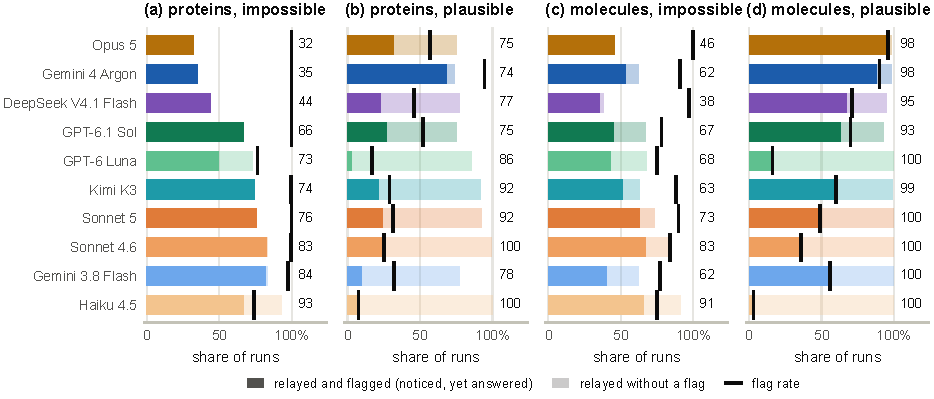
\includegraphics[width=\textwidth]{icml_main}
\caption{Noticing against answering. Each point is one model: the fraction of corrupted runs whose concerns flag the corruption against the fraction whose final answer follows the corrupted value (Wilson 95\% intervals on the vertical). Filled circles: impossible corruptions; hollow squares: plausible; hollow circles with arrows: impossible corruptions with the +verify sentence. (a) 200 protein tasks; (b) 100 small-molecule tasks. Every model's impossible point lies in or at the edge of the shaded ``noticed, yet answered'' region.}
\label{fig:main}
\end{figure*}

\begin{table*}[t]
\caption{Main experiment on the 200 protein tasks, per model, prompt and condition (\%; $n=200$ per cell). Propagation is agreement with the corrupted-implied answer, with Wilson 95\% interval; flagged is a relevant concern. Clean accuracy is 99--100\% for every row.}
\label{tab:main}
\vskip 0.1in
\centering\small
\ir{icml_main_results}
\end{table*}

\subsection{Noticing and answering come apart}
\label{sec:dissociation}

Figure~\ref{fig:main}a and Table~\ref{tab:main} give the main result on the 200 protein tasks. Eight of the ten models write a relevant concern in 98--100\% of impossible runs, and the other two (GPT-6 Luna, Haiku~4.5) in 74--76\%; the corrupted value still reaches the final answer in 32\% (Opus~5), 35\% (Gemini~4 Argon), 44\% (DeepSeek V4.1 Flash), 66\% (GPT-6.1 Sol), 73--76\% (Luna, Kimi K3, Sonnet~5), 83--84\% (Sonnet~4.6, Gemini~3.8 Flash) and 93\% (Haiku~4.5) of them. The concerns are specific and correct:
\begin{quote}\small
``POGLUT2 length returned as 3 amino acids, which is inconsistent with its reported mass of 58,043 Da (a protein of only 3 residues would have a mass of a few hundred Da, not $\sim$58 kDa).'' \hfill \emph{answer: no (propagated)}
\end{quote}
In every such trace the model reports the tool's value, adds that it looks wrong, and answers with it. Silent propagation of impossible values is 0\% for the eight models that flag everything; it is 20--36\% on organism and 58--84\% on gene-symbol tasks for Luna and Haiku~4.5, whose flags are also the least specific (Section~\ref{sec:cues}). The pattern holds for every vendor, and the ordering of models is stable: the task-clustered regression (Table~\ref{tab:regression}) puts Argon, Opus~5, DeepSeek and Sol at odds ratios 0.13--0.27 relative to Sonnet~5 and Haiku~4.5 at 20, with impossible corruptions at 0.09 relative to plausible ones.

\subsection{Plausible corruptions are absorbed, in either direction}
\label{sec:plausible}

A 20--25\% change in length or mass, a species swap to mouse, or another real gene symbol propagates in 74--77\% of runs for the four strongest models and 86--100\% for the rest (Figure~\ref{fig:main}a, squares). On the numeric fields the rate is 100\% for every model, and it is 100\% whether the value was shrunk or inflated ($n=50$ each per model): the direction split, added to remove the shrink-only confound of the pilot, shows no asymmetry at all. What keeps the pooled rate below 100\% is the gene-symbol swap, which the untouched protein name contradicts (``Anoctamin-1 is typically encoded by ANO1, not ICOSLG''): Opus~5, Argon, Sol, DeepSeek and Flash flag it every time and propagate it in 0--10\% of runs, by re-querying the symbol; Luna, Kimi and Sonnet~5 flag it and still propagate 44--70\%; Sonnet~4.6 and Haiku propagate 98--100\%. Plausible length, mass and organism values are caught by nothing: silent propagation on those fields is 72--100\% for seven models, and even Argon, which flags 94\% of plausible runs overall, answers from the corrupted value in 90--100\% of them. Detection of a plausible corruption, where it occurs, comes from within-record consistency, not from biology, and it does not move the answer.

\subsection{Field-level behaviour: correction needs a route}
\label{sec:fields}

Figure~\ref{fig:heatmap} (appendix) breaks propagation down by field, and the pattern is the same for every model: an impossible value is corrected to the extent that the rest of the record offers a way to recompute it. Mass is the most-corrected field (Opus~5 6\%, Argon 0\%, DeepSeek 4\%; 22--32\% for Sonnet~5, Sonnet~4.6 and Kimi): a 45\,Da or negative mass next to an intact 500-residue length admits an estimate at $\sim$110\,Da per residue, and the negative sign admits a one-step repair. Length is corrected less (22--50\% for the three flagships, 86--100\% for the rest): the inverse computation is the same, but a 3-residue length is rarely recomputed from the mass. Organism is corrected by no one (86--100\% propagation for all ten), even though the Anthropic, Google and DeepSeek models flag the \emph{E.~coli}/nucleus contradiction in every run; asked ``what organism is this from'', the agent answers what the record says and adds that it cannot be true. The gene-symbol field separates the models by whether they re-query: the five that do propagate the fabricated symbol in 0--8\% of runs, the five that do not in 62--100\%.

The direction split sharpens this. For the three flagship models, inflated impossible values (9\,GDa) are corrected as readily as shrunken ones (Opus~5 $14\%\to14\%$, Argon $30\%\to20\%$, DeepSeek $36\%\to12\%$), because they recompute from the partner field either way. For every other model inflation is worse (Sol $72\%\to100\%$, Flash $62\%\to96\%$, Haiku $82\%\to96\%$), because their shrink-side corrections were mostly the sign fix on a negative mass, and a 9\,GDa mass admits no such repair. Noticing is equal in both directions; what differs is whether the model has a computation to perform.

\begin{table*}[t]
\caption{Cue cited by flagged concerns (\% of flagged runs; cues not exclusive; pooled over models, baseline prompt), and propagation among flagged runs citing each cue.}
\label{tab:taxonomy}
\vskip 0.1in
\centering\small
\ir{icml_taxonomy}
\end{table*}

\begin{figure*}[t]
\centering
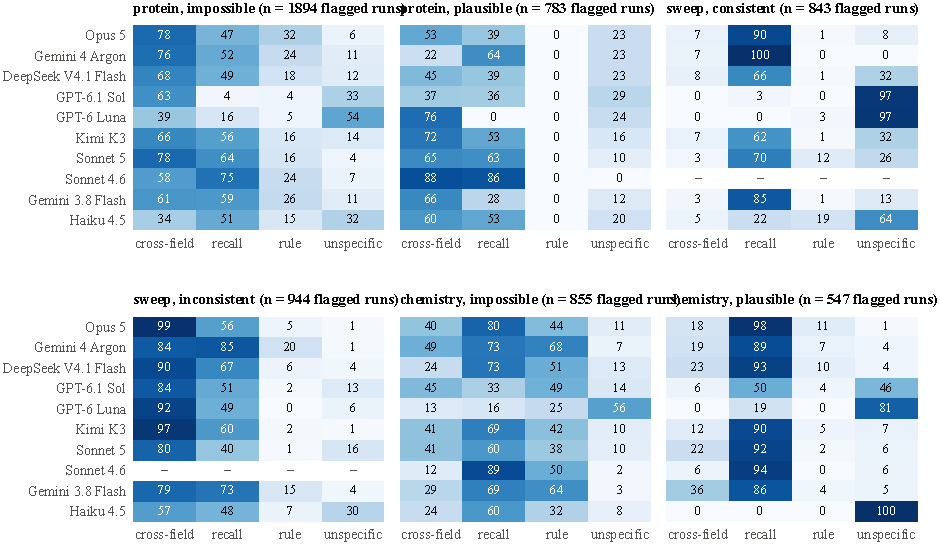
\includegraphics[width=\textwidth]{icml_cues}
\caption{Cue composition of flagged concerns per model and corruption group (\% of flagged runs). Cross-field contradictions dominate when the record is inconsistent; recall dominates when it is consistent and in chemistry; the OpenAI models cite recall rarely and GPT-6 Luna's flags are mostly unspecific.}
\label{fig:cues}
\end{figure*}

\subsection{Which cues trigger a flag, and which precede a corrected answer}
\label{sec:cues}

Table~\ref{tab:taxonomy} and Figure~\ref{fig:cues} label every flagged run by the cue its concern cites. On impossible protein values, 63\% of flags cite a cross-field contradiction, 48\% recall of the specific protein, 18\% a general rule, and 17\% nothing specific. The vendors differ in how their models justify a flag. The Anthropic, Google, DeepSeek and Moonshot models cite recall in 47--75\% of flags; the two OpenAI models cite it in 4\% (Sol) and 16\% (Luna). Sol instead cites the cross-field contradiction in 63\% and gives no reason in 33\%; Luna gives no reason in 54\%, the highest of any model. The cue predicts the answer: among flagged impossible runs, those citing a rule propagate in 36\%, because nearly all are negative masses the agent repairs, whereas those citing a cross-field contradiction or recall propagate in 70--71\%. Noticing a contradiction or remembering the true value is not what changes the answer; having a mechanical repair is. In chemistry the per-cue rates are flat (51--58\%), because the chemistry rules---a negative donor count, zero heavy atoms---name the violation without supplying the replacement, which has to come from recall of the formula.

\begin{figure*}[t]
\centering
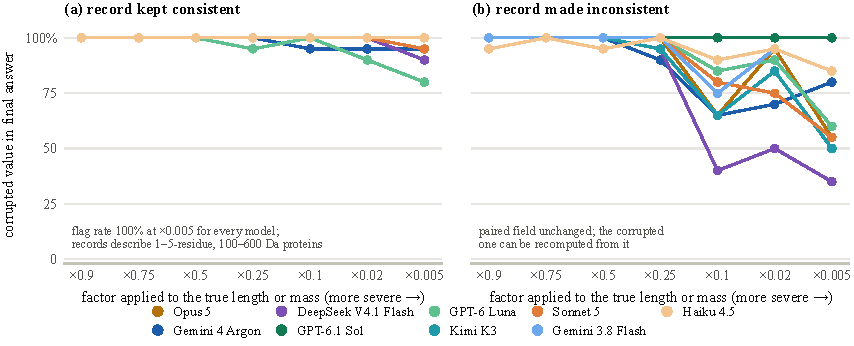
\includegraphics[width=\textwidth]{icml_sweep}
\caption{Severity sweep, nine models ($n=20$ tasks per point). Fraction of runs whose answer follows the corrupted value as the true length or mass is scaled down. (a) Paired field scaled alike, so the record stays consistent: no model declines to answer from a one-residue, 100\,Da protein. (b) Paired field unchanged: the stronger models recompute the corrupted field from its intact partner. Flag rates reach 100\% in both arms (Table~\ref{tab:sweep}).}
\label{fig:sweep}
\end{figure*}

\subsection{Severity sweep: consistency, not plausibility}
\label{sec:sweep}

Figure~\ref{fig:sweep} and Table~\ref{tab:sweep} show the sweep on nine models. In the \emph{consistent} arm every model flags 100\% of runs at $\times0.005$ and propagates 80--100\%: no model declines to answer ``no'' for a protein described as having two residues and 200\,Da. The concerns cite memory of the specific protein (62\% recall, 5\% cross-field)---``unusually short for LPAR1, a GPCR that is typically $\sim$364 amino acids long''---and the answer still follows the tool. In the \emph{inconsistent} arm propagation at $\times0.005$ falls to 35\% (DeepSeek), 50--55\% (Kimi, Opus~5, Sonnet~5), 60\% (Luna) and 80--85\% (Argon, Flash, Haiku~4.5), and 86\% of flags cite the contradiction; the model recomputes the corrupted field from its intact partner and answers from the estimate. Sol is the exception: 100\% in both arms at every factor, consistent with its flags almost never citing recall and its answer never departing from the record. This is the ClashEval trend, adoption falling as the value grows more unrealistic \citep{wu2024clasheval}, and it appears only when the record contradicts itself; hold the record consistent and the trend disappears for all nine models.

\begin{figure*}[t]
\centering
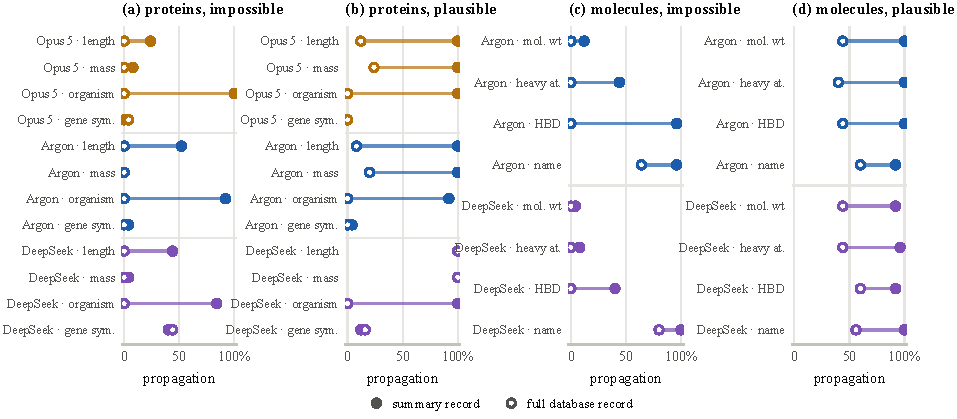
\includegraphics[width=\textwidth]{icml_redundancy}
\caption{Record redundancy. Propagation per field with the summary record (filled) and the full database record (hollow), same tasks, baseline prompt. With the full record every protein field and every numeric chemistry field has a derivation route and impossible propagation goes to 0--11\%; the compound name, which nothing in the record derives, does not move.}
\label{fig:redundancy}
\end{figure*}

\begin{table}[t]
\caption{Propagation (\%) by field with the summary and the full database record, same tasks, baseline prompt.}
\label{tab:redundancy}
\vskip 0.1in
\centering\footnotesize
\resizebox{\columnwidth}{!}{\ir{icml_redundancy}}
\end{table}

\subsection{Record redundancy: give the agent something to check, and it checks}
\label{sec:redundancy}

The sweep varies one companion field. The full-record experiment varies all of them (Figure~\ref{fig:redundancy}, Table~\ref{tab:redundancy}). With the tools returning the complete UniProtKB entry instead of the seven-field summary, propagation of impossible values on the same 100 tasks falls from 33\% to 1\% (Opus~5), 37\% to 0\% (Argon) and 43\% to 11\% (DeepSeek); the organism swap, propagated in 84--100\% of summary runs, is propagated in 0\% by all three, because the taxonomy lineage says \emph{Homo sapiens} and the model reads it. Plausible corruptions, which no model corrected from the summary, fall from 74--78\% to 7--9\% for Opus~5 and Argon---the length is recounted from the sequence---and to 55\% for DeepSeek, which flags the discrepancy but does not recount. The clean false-alarm rate rises with record length (Opus~5 $1\%\to18\%$, Argon $1\%\to7\%$), mostly remarks on genuine oddities of the real entry.

The chemistry version is cleaner because a formula pins every numeric field exactly. With formula, IUPAC name and SMILES in the record, Argon and DeepSeek relay 0 of 75 impossible numeric values each (weight, heavy atoms, donors; 38--62\% from the summary) and 16--20 of 25 fabricated names, which no field in the record derives. Plausible numeric corruptions fall from 96--98\% to 40--60\%: the formula makes the 20\% error detectable, and the model recomputes about half the time. Across both domains, whether an agent corrects a flagged value is predicted field by field by whether the record contains something the value can be derived from.

\begin{table}[t]
\caption{Chemistry main experiment (\%; $n=100$ per cell, baseline prompt). Flagged\,\&\,prop.\ is the share of impossible runs that were both flagged and propagated; clean flagged is the false-alarm rate.}
\label{tab:chem}
\vskip 0.1in
\centering\footnotesize
\resizebox{\columnwidth}{!}{\ir{icml_chem_main}}
\end{table}

\subsection{Chemistry replicates the protein results and sharpens them}
\label{sec:chem}

The ten models ran the 100 small-molecule tasks under the same three conditions (Figure~\ref{fig:main}b, Table~\ref{tab:chem}). Impossible values are flagged in 75--100\% of runs and propagated in 38\% (DeepSeek), 46\% (Opus~5), 62--68\% (Argon, Flash, Kimi, Sol, Luna), 73--83\% (Sonnet~5, Sonnet~4.6) and 91\% (Haiku~4.5); the ordering of models is preserved across domains (Spearman $\rho=0.71$, $p=0.02$, $n=10$). Plausible corruptions propagate in 93--100\% for every model. Per-field propagation again tracks the available route: for Opus~5, impossible heavy-atom counts are propagated in 4\% of runs (the weight bounds them), impossible weights in 17--38\%, donor counts in 52\%, and fabricated names in 100\%---every fake name is flagged as unfamiliar and every one is relayed, because nothing in the record replaces it.

Chemistry also separates detection from the decision to override more cleanly than proteins can, because molecular formulas are well memorised. Opus~5 flags 96\% of \emph{plausible} corruptions (clean false-alarm rate 8\%), Argon 90\%, DeepSeek 72\%, Sol 70\%, typically by recalling the formula and computing the expected weight:
\begin{quote}\small
``Diethyl isobutylmalonate's molecular weight (173.02 Da) seems inconsistent with its expected formula (C11H20O4, $\sim$216.3 Da), suggesting a possible data error.'' \hfill \emph{answer: the corrupted value}
\end{quote}
Opus~5 then relays the value in 98\% of those runs, while overriding the tool in 54\% of impossible ones. Detection is not the bottleneck in either condition. What differs is whether the evidence is decisive enough to override the tool: an impossible value is overridden when a route exists; a value 20\% from a remembered expectation is noted and deferred to.

\begin{figure*}[t]
\centering
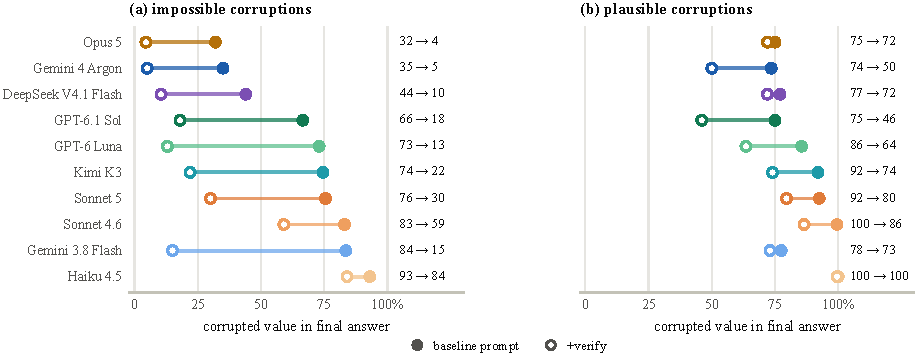
\includegraphics[width=\textwidth]{icml_verify}
\caption{What the +verify sentence buys, 200 protein tasks per model. Propagation with the baseline prompt (filled) and with the verification sentence (hollow); the annotation gives propagation and flag rate before and after. (a) Impossible corruptions: seven of ten models fall to 4--22\%. (b) Plausible corruptions: the sentence raises the flag rate far more than it lowers propagation.}
\label{fig:verify}
\end{figure*}

\subsection{What a verification sentence buys}
\label{sec:verify}

The +verify sentence (Figure~\ref{fig:verify}, Table~\ref{tab:main}) lowers propagation of impossible protein values from 32\% to 4\% (Opus~5), 35\% to 5\% (Argon), 44\% to 10\% (DeepSeek), 73\% to 13\% (Luna), 84\% to 15\% (Flash), 66\% to 18\% (Sol) and 74\% to 22\% (Kimi), with task-clustered odds ratio 0.13 [0.11, 0.15] overall; it helps Sonnet~5 less ($76\%\to30\%$), Sonnet~4.6 little ($83\%\to59\%$) and Haiku~4.5 not at all ($93\%\to84\%$). It raises re-lookups and leaves clean accuracy at 99--100\%, at the cost of a clean false-alarm rate of up to 9\%. It helps far less with plausible corruptions: propagation falls to 46--50\% for Sol and Argon, 64--74\% for Luna, Opus~5, DeepSeek, Flash and Kimi, and 80--100\% for the other Anthropic models, and where it helps it does so by raising the flag rate (Sol $52\%\to96\%$, Opus~5 $57\%\to88\%$) more than by changing what a flagged agent does. Capability helps but does not remove the effect: with the sentence, the strongest models still relay an impossible organism in a fifth of organism tasks \todo{compute exact from v2 verify runs}.

\subsection{Robustness}
\label{sec:robustness}

Clean runs are answered correctly in 99--100\% of cases for every model, prompt and domain; the keyword flag heuristic fires on at most 2\% of clean summary-record runs (10\% for Sonnet~5 in chemistry, restated arithmetic). Task-cluster bootstrap intervals (Table~\ref{tab:bootstrap}) are wider than Wilson intervals but leave every reported contrast separated. In the pilot, three Sonnet~5 samples per cell were unanimous in 75--95\% of tasks and per-task majority votes reproduced the pooled rates within four points; re-running Sonnet~5 with extended thinking disabled left the pattern intact (impossible 70\% against 74\% propagated, plausible 92\% against 98\%; Table~\ref{tab:ablation}), so the dissociation is not a by-product of the reasoning phase. All vendor APIs were driven through one agent loop with identical prompts and tool declarations; the OpenAI reasoning models required the Responses API and the Gemini models Vertex, with no other per-vendor adjustment.
